
\chapter{The Standard Model of particle physics}\label{sec:SM}
This chapter introduces the Standard Model of particle physics which describes the family of elementary particles and the three of the four fundamental
forces of Nature with corresponding mediators. After that, the gauge symmetry is briefly expressed. Then, the Drell-Yan process is introduced in details due to its importance in this thesis. In Addition, the photon induced process is also shortly discussed. Finally, the effective field theory which will be used in this thesis is presented.
\section{The elementary particles}\label{subsec:elem_particle}
It has been long time for people to understand what are the basic objects which constitute our world. From Demokritos (470-380 BC) who thought matter was built of discrete building blocks to John Dalton (1766-1844) who came up with the matter made of atoms. In the early 1900's J.J. Thomson proposed a so called ``plum pudding model'' which assumes the atom was a uniform sphere of positively charged matter in which electrons were embedded. However in 1910 Ernest Rutherford and his colleagues performed $\alpha$ ray scattering experiments and found that the whole mass and all positive charges of the atom were concentrated in a minute space at the centre which is called ``nucleus''. After the discovery of the neutron in 1932 by James Chadwick, models for a nucleus composed of protons and neutrons were quickly developed by Dmitri Ivanenko and Werner Heisenberg. Furthermore in 1968 the deep inelastic scattering experiments at the Stanford Linear Accelerator Center provided the first convincing evidence of the reality of quarks in the proton or neutron. In the Standard Model (SM) \cite{David_Griffiths,Francis_Alan,Morii_Lim} the quarks are the elementary particles and there are six different kinds of flavors for the quarks called up (u), down (d), charm (c), strange (s), top (t), and bottom (b). The mass, charge, and spin of the quarks are shown in Table \ref{tab:quarks}, here the e means one electron's charge which equals $\mathrm{1.6\times10^{-19}~C}$. The quarks are categorized in there generations according to their masses and charges. Besides it is verified that the quarks have another property which is called the ``color charge'', a quark can be ``Red'' or ``Blue'' or ``Green''. Moreover all the quarks have its anti-quark partner which has opposite quantum numbers with regard to the quark including flavor, charge, and color charge. Therefore there are $\mathrm{6~(flavor)~\times~3~(color)~\times~2~(anti-quark)~=~36}$ kinds of quarks in the SM and all the hadrons are composed by quarks or anti-quarks. For meson it is composed by $\mathrm{q\bar{q}}$ and for baryon it is composed by $\mathrm{qqq}$ or $\mathrm{\bar{q}\bar{q}\bar{q}}$.
 \begin{table}[!hbpt]
 \begin{center}
 \begin{tabular}{|c|c|c|c|c|}
 \hline
 Generation           & Quark         & Charge      &Spin      & Mass \\ \hline
 First                & up quark (u)  & 2/3 e     &1/2       & $2.3^{+0.7}_{-0.5}$ MeV \\
                      & down quark (d)& -1/3 e    &1/2       & $4.8^{+0.5}_{-0.3}$ MeV \\ \hline
 Second               & charm quark (c)& 2/3 e    &1/2       & $1.275 \pm 0.025$ GeV \\
                      & strange quark (s)& -1/3 e &1/2       & $95\pm 5$ MeV \\  \hline
 Third                & top quark (t)    & 2/3 e  &1/2       & $173.21\pm 0.51 \pm 0.71$ GeV \\
                      & bottom quark (b) & -1/3 e &1/2       & $4.66 \pm 0.03$ GeV \\ \hline
 \end{tabular}
 \end{center}
 \caption{Quarks and their properties \cite{Olive:2016xmw}.\label{tab:quarks}}
 \end{table}

\begin{table}[!hbpt]
\begin{center}
\begin{tabular}{|c|c|c|c|c|}
\hline
Generation & Lepton                               & Charge &Spin & Mass \\ \hline
First      & electron ($\mathrm{e}$)              & -e   &1/2  & 511 MeV\\
           & electron neutrino ($\mathrm{\nu_e}$) & 0      &1/2  & $<$ 2 eV\\ \hline
Second     & muon ($\mathrm{\mu}$)                & -e   &1/2  & 105.67 MeV\\
           & muon neutrino ($\mathrm{\nu_{\mu}}$) & 0      &1/2  & $<$ 2 eV\\ \hline
Third      & tau ($\mathrm{\tau}$)                & -e   &1/2  & 1776.99 MeV\\
           & tau neutrino ($\mathrm{\nu_{\tau}}$) & 0      &1/2  & $<$ 2 eV\\ \hline
 \end{tabular}
 \end{center}
 \caption{Properties of the leptons in the three generations. Neutrinos are assumed to have zero mass in SM but by the observation of neutrino's oscillations the upper limits on their masses are set \cite{Olive:2016xmw}.\label{tab:leptons}}
 \end{table}

Similar to the quark family, there is a lepton family and the most common lepton is the electron which exists as a cloud out of nucleus to form an atom. All the leptons are shown in Table \ref{tab:leptons} with their charges, spins, and masses. They are electron ($\mathrm{e}$), electron neutrino ($\mathrm{\nu_e}$), muon ($\mathrm{\mu}$), muon neutrino ($\mathrm{\nu_{\mu}}$), tau ($\mathrm{\tau}$), and tau neutrino ($\mathrm{\nu_{\tau}}$). The leptons are also categorized into three generations and each generation has its own lepton flavor. The first generation has electron flavor, the second generation has muon flavor, and the third generation has tau flavor. For neutrinos they are always left handed and they are very hard to be detected because of the very weak interaction between the matter and neutrinos. In SM the neutrinos are assumed to be massless while in experiment we have observed the neutrino oscillations which means the neutrinos have masses, so the study of neutrinos may bring us the new theory beyond the SM.
 Similar with the quarks, all the leptons also have theirs anti-particle partners which own the opposite quantum numbers. While unlike the quarks, the leptons do not have color charge property. Therefore there are $6~\times~2~=~12$ kinds of leptons in SM.

Now that all the spin 1/2 (fermion) elementary particles in SM have been introduced, the interactions between these particles and the mediators will be discussed in the next section.



\section{The fundamental interactions}\label{subsec:fund_interaction}
It is well known that there are four characteristic interactions among fundamental particles.
\begin{enumerate}
\item Electromagnetic interaction : It is mediated by massless photon ($\mathrm{m_{\gamma}~=~0}$) with spin = 1 among charged particles. Because of the massless of photon the interacting range of electromagnetic interaction is infinite. The theory to describe the electromagnetic interaction is quantum electrodynamics (QED) which has been well understood.  QED is renormalizable, for example the divergence from vacuum polarization and higher order loop contributions can be absorbed into the physical charge of particle. The coupling constant is $\mathrm{\alpha~=~\frac{e^{2}}{4\pi\varepsilon_{0}\hbar c}} ~\simeq ~ \frac{1}{137}$ which characterizes the strength of the coupling of charged particle with the electromagnetic field. Because of the smallness of $\mathrm{\alpha}$, the perturbation development works well for QED. 
    %Besides the $\mathrm{\alpha}$ is running, the coupling will increase when the energy scale of interaction increases, but the difference is very small for wide energy range.
\item Strong interaction : It is mediated by massless gluons ($\mathrm{m_{g}~=~0}$) with spin = 1. This interaction can only happen between quarks and gluons. The theory that describes the strong interaction is called quantum chromodynamics (QCD). For strong interaction the coupling strength is also running but in an opposite way as the electromagnetic interaction, which means that the coupling will decrease when the interaction energy increases. Because of that there is one special phenomenon for strong interaction called ``asymptotic freedom'' which means quarks and gluons behave like free particles when the interaction energy is very high. At high energy the perturbation theory works well because of ``asymptotic freedom'' but it is not the case at low energy (below the GeV). Therefore there are still a lot of works needed to be done for understanding QCD process at low energy. Another special phenomenon of the strong interaction is called the ``color confinement'', which means there are no free quarks in the world. The quarks need to be grouped to form a colorless hadron. For instance the baryon is formed by red, green, and blue quarks and the meson is formed by red and anti-red quarks or blue and anti-blue quarks or green and anti-green quarks.
\item Weak interaction : It is mediated by massive weak bosons ($\mathrm{m_{W^{\pm}}~\cong~80.4~GeV,}$ \\ $\mathrm{m_{Z}~\cong~91.2~GeV}$) with spin = 1. Because of the heavy mediator, its interacting range is very short, which is $\sim 10^{-18}$ m. The coupling strength of weak interaction is the weakest among electromagnetic and strong interactions. Although the coupling strength is small, some processes can only happen via weak interaction like flavor changing or neutrino involved processes.
\item Gravitational interaction : It is mediated by massless gravitons ($\mathrm{m_{G}~=~0}$) with spin = 2 among all massive particles. Because of its very small coupling strength we normally do not consider gravitational interaction in high energy physics. In macroscopic world the gravitation is important, such as it makes an apple falling.
\end{enumerate}

The summary of interaction range, relative strength, and mediator for the four fundamental interactions is shown in Table \ref{tab:interactions}.
Last but not least, in the SM the origin of mass of the elementary particles is coming from interactions between particles and the Brout-Englert-Higgs scalar field  (the so called ``Higgs'' boson). In 2012 the ATLAS \cite{Aad:2012tfa} and CMS \cite{Chatrchyan:2012xdj} experiments observed such a particle and the mass is $\sim \mathrm{125~GeV}$.

The summary of all elementary particles, force carries, and Higgs boson is shown in Figure \ref{fig:SM}.

 \begin{table}[!hbpt]
 \begin{center}
 \begin{tabular}{|c|c|c|c|}
 \hline
 Interaction & Range & Relative strength & Mediators \\
 \hline
 Strong & $10^{-15}$ m & 1 &  8 gluons ($\mathrm{g}$) \\
 \hline
 Electromagnetic & $\infty$ & $10^{-3}$ & photon ($\gamma$) \\
 \hline
 Weak &  $10^{-18}$ m & $10^{-14}$ & $\mathrm{W^+}$, $\mathrm{W^-}$, $\mathrm{Z}$ \\
 \hline
 Gravitational & $\infty$ & $10^{-43}$ & graviton (G) ? \\
 \hline
  \end{tabular}
 \end{center}
 \caption{Range, relative strength with respect to the strong force, and mediators of the four fundamental interactions. The gravitational force is not included in the SM, and gravitons are hypothetical particles.
 \label{tab:interactions}
}
 \end{table}

\begin{figure}[h!]
 \begin{center}
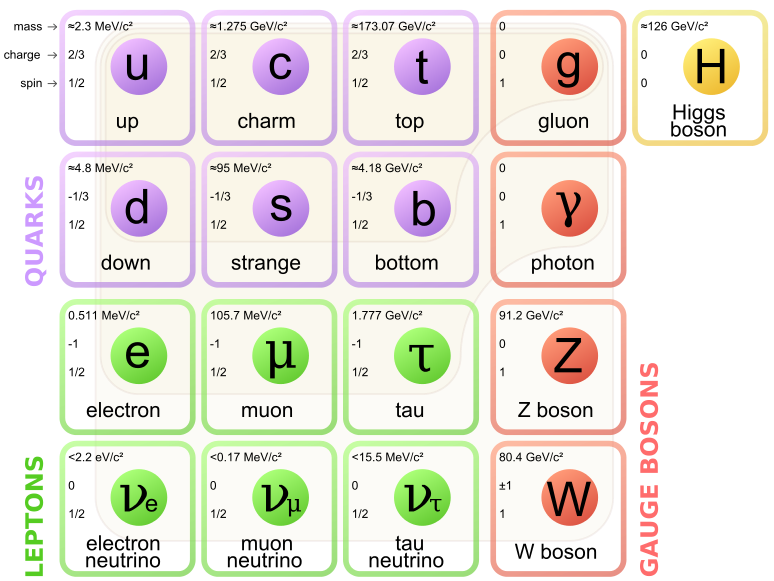
\includegraphics[width=0.75\textwidth]{figures/theory/sm.png}
\caption{Overview of the Standard Model constituents: the quarks and leptons, the gauge bosons and the Higgs boson.}
  \label{fig:SM}
 \end{center}
\end{figure}

An introduction about the Feynman calculus is presented in Appendix \ref{subsec:Feynman}. Besides, more detailed introductions about the QED and the QCD are presented in Appendix \ref{subsec:QED} and Appendix \ref{subsec:QCD}, respectively. The group theory is briefly introduced in Appendix \ref{sec:Groups}.




\clearpage
\section{Gauge symmetries: a brief introduction}\label{sec:Gauge}
\textit{The formulas in this section are from book \cite{Quark_Lepton}.}
\subsection*{The Lagrangian}\label{subsec:Lagrangian}

As we know, in classic physics, the motion equation of a particle can be obtained from the Lagrange's equation
\begin{equation}
\frac{d}{dt}(\frac{\partial L}{\partial \dot{q_i}}) - \frac{\partial L}{\partial q_i}=0
\label{eq:Lagrangian}
\end{equation}
where the $q_i$ are the generalized coordinates of the particle, $t$ is the time variable and $\dot{q_i}=dq_i/dt$. The $L\equiv T-V$, where $T$ is kinetic energy of the particle and $V$ is the potential energy of the particle. The Lagrange's equation \ref{eq:Lagrangian} can be extended from describing the motion of one particle to describe the motion of a field $\phi(t,\mathbf{x})$ (which has a value at every point in space that changes in time) by replace $q_i$ and $\dot{q_i}$ with $\phi$ and $\partial\phi/\partial x_\mu$ respectively, here the $x_\mu\equiv(t,\mathbf{x})$. Therefore, we obtained the Lagrange's equation for field $\phi$ as
\begin{equation}
\frac{\partial}{\partial x_\mu}(\frac{\partial \mathcal{L}}{\partial (\partial\phi/\partial x_\mu)}) - \frac{\partial \mathcal{L}}{\partial\phi}
=\frac{\partial}{\partial t}(\frac{\partial \mathcal{L}}{\partial (\partial\phi/\partial t)})+\sum_{i=1}^{3}\frac{\partial}{\partial x_i}(\frac{\partial \mathcal{L}}{\partial (\partial\phi/\partial x_i)}) - \frac{\partial \mathcal{L}}{\partial\phi}=0,
\label{eq:Euler_Lagrangian}
\end{equation}
which is called Euler-Lagrange equation and the $\mathcal{L}$ is Lagrangian density with
$$L=\int \mathcal{L} d^{3}x.$$
Usually we call $\mathcal{L}$ itself the Lagrangian.

For example, the Dirac Lagrangian (which describes the spin $\frac{1}{2}$ particle in quantum mechanics) is
\begin{equation}
\mathcal{L}=i\overline{\psi}\gamma_\mu\partial^{\mu}\psi-m\overline{\psi}\psi
\label{eq:Lagrangian_Dirac}
\end{equation}
where $\psi$ is the particle field and $\overline{\psi}\equiv\psi^{\dag}\gamma^{0}$, $m$ is the mass of the particle, the $\partial^{\mu}=(\frac{\partial}{\partial t}, -\nabla)=(\frac{\partial}{\partial t}, -\frac{\partial}{\partial x_1}, -\frac{\partial}{\partial x_2}, -\frac{\partial}{\partial x_3})$, $\gamma_\mu=(\gamma_0, \gamma_1, \gamma_2, \gamma_3)$ are the gamma matrices:

\begin{equation}
\begin{split}
&\gamma_0=\begin{pmatrix} 1 & 0 \\ 0 & -1 \end{pmatrix},~
\gamma_i=\begin{pmatrix} 0 & -\sigma_i \\ \sigma_i & 0 \end{pmatrix} ~~\mathrm{with}~i~=~1,~2,~3\\
&\sigma_1=\begin{pmatrix} 0 & 1 \\ 1 & 0 \end{pmatrix},~\sigma_2=\begin{pmatrix} 0 & -i \\ i & 0 \end{pmatrix},~\sigma_3=\begin{pmatrix} 1 & 0 \\ 0 & -1 \end{pmatrix}
\end{split}
\label{eq:gamma_mu}
\end{equation}

\subsection*{Symmetry and conservation}\label{subsec:Sym_con}

The first person who linked symmetry with conservation law is Emmy Noether \cite{Noether_Emmy}. She pointed out that each symmetry (which means the physics or the Lagrangian is invariant under this operation) corresponds to one conserved quantity. For example, the symmetries of transitions, time displacements, and rotations lead to the conservation of momentum, energy and angular momentum. An example about ``internal'' symmetry is given below.

Suppose we change the phase of electron field by
\begin{equation}
\psi\rightarrow e^{i\alpha}\psi,
\label{eq:global_phase}
\end{equation}
where $\alpha$ is space and time independent. It is easily to see that this operation is a symmetry operation (usually called global $U(1)$ symmetry, because all these kind of operations with different $\alpha$ value form a unitary group with one group generator, the global means $\alpha$ is space and time independent) due to the invariance of Lagrangian (see Equation \ref{eq:Lagrangian_Dirac}). From Noether's theorem we know there is a conserved quantity corresponding to this symmetry.

According to the property of $U(1)$ group, when $\alpha$ is infinitesimal the Equation \ref{eq:global_phase} can be written as
\begin{equation}
\psi\rightarrow (1+i\alpha)\psi.
\label{eq:global_phase_1}
\end{equation}
and by asking the invariance of Lagrangian we get
\begin{equation}
0=\delta\mathcal{L}=\frac{\partial}{\partial \psi}\delta\psi+\frac{\partial}{\partial (\partial_\mu \psi)}\delta(\partial_\mu \psi)+\frac{\partial}{\partial \overline{\psi}}\delta\overline{\psi}+\frac{\partial}{\partial (\partial_\mu \overline{\psi})}\delta(\partial_\mu \overline{\psi})
\label{eq:global_phase_2}
\end{equation}
and finally we can get can a conserved current from
\begin{equation}
\partial_\mu j^{\mu}=0,
\label{eq:global_phase_3}
\end{equation}
where
\begin{equation}
j^{\mu}=\frac{ie}{2}(\frac{\partial}{\partial (\partial_\mu \psi)}\psi-\overline{\psi}\frac{\partial}{\partial (\partial_\mu \overline{\psi})})=-e\overline{\psi}\gamma^{\mu}\psi.
\label{eq:global_phase_4}
\end{equation}

It can be proved that the conserved current $j^{\mu}$ leads to the charge conservation of the particle.


\subsection*{$U(1)$ local gauge symmetry}\label{subsec:U1_local}

As we know, in previous section, the Lagrangian (Equation \ref{eq:Lagrangian_Dirac}) is invariant under $U(\alpha)$ operation, while it will not be the case for local operator $U(\alpha(t,\mathbf{x}))$ which is time and space dependent. However, the real Lagrangian should be invariant with $U(\alpha(t,\mathbf{x}))$, as we know the observation $|\langle\psi|\psi\rangle|^2=|\langle\psi|U^{\dag}U|\psi\rangle|^2$ do not dependent with the phase.

In order to maintain the Lagrangian is invariant under $U(\alpha(t,\mathbf{x}))$, it is needed to replace derivative $\partial_\mu$ by $D_\mu$ with
\begin{equation}
D_\mu\equiv\partial_\mu-ieA_\mu
\label{eq:D_mu}
\end{equation}
where $A_\mu$ transforms as
\begin{equation}
A_\mu\rightarrow A_\mu+\frac{1}{e}\partial_\mu\alpha.
\label{eq:A_mu}
\end{equation}

Therefore, the updated Lagrangian will be
\begin{equation}
\mathcal{L}=i\overline{\psi}\gamma^{\mu}D_\mu \psi-m\overline{\psi}\psi=\overline{\psi}(i\gamma^{\mu}\partial_\mu-m)\psi+e\overline{\psi}\gamma^{\mu}\psi A_\mu,
\label{eq:Lagrangian_Dirac_new}
\end{equation}
which means there is an interaction between the field $\psi$ and field $A_\mu$. Actually, it can be proved that the $A_\mu$ can be regarded as the photon and after include the kinetic term of the photon (not for the mass term which will break the symmetry) the final Lagrangian for QED is
\begin{equation}
\mathcal{L}_{QED}=\overline{\psi}(i\gamma^{\mu}\partial_\mu-m)\psi+e\overline{\psi}\gamma^{\mu}\psi A_\mu-\frac{1}{4}F_{\mu\nu}F^{\mu\nu}
\label{eq:Lagrangian_QED}
\end{equation}
with
\begin{equation}
F_{\mu\nu}=\partial_\mu A_\nu-\partial_\nu A_\mu
\label{eq:F_tensor}
\end{equation}

We have seen that after asking the local $U(1)$ symmetry, a massless gauge boson, the photon, is created.

\subsection*{$SU(3)$ local gauge symmetry}\label{subsec:U3_local}

As we know, the quark has three colors (R, G, B) and the Lagrangian
\begin{equation}
\mathcal{L}=\overline{q_i}(i\gamma^{\mu}\partial_\mu-m)q_i,~~\mathrm{with}~i~=~1,~2,~3,
\label{eq:L_quarks}
\end{equation}
where the $q_1$, $q_2$, $q_3$ denote the three color fields, should be invariant under the color phase transformation (R $\rightleftarrows$ G $\rightleftarrows$ B). This is because we really can't distinguish the exact color of one quark. This color phase transformation can be represented by 3 $\times$ 3 traceless unitary matrices U, and all these matrices form a $SU(3)$ (``S'' means special because of the zero trace of the matrices) group with 8 generators. The transformation of the quark field under the color phase change can be written as
\begin{equation}
q(t,\mathbf{x})\rightarrow Uq(t,\mathbf{x})\equiv e^{i\alpha_a(t,\mathbf{x})T_a}q(t,\mathbf{x}),
\label{eq:Quark_transfer}
\end{equation}
where a summation over suffix $a$ from 1 to 8 is implied, the $T_a$ are a set of linearly independent traceless 3 $\times$ 3 matrices, and the $\alpha_a$ are the group parameters. Because not all generators $T_a$ commute with each other (e.g. $T_aT_b\neq T_bT_a$), this group is non-Abelian. The conventional choice of $T_a$ matrices are the $\lambda_a /2$ (know as Gell-Mann $\lambda$ matrices, see Equation \ref{eq:lambda_matrices}). It can be proved that the commutator of any two $T_a$ follows
\begin{equation}
[T_a, T_b]=if_{abc} T_c,
\label{eq:Commutator_T}
\end{equation}
where $f_{abc}$ are real constant, called the structure constants of the group.

In order to impose the $SU(3)$ color local invariance of the Lagrangian \ref{eq:L_quarks}, we can use the same method described in Section \ref{subsec:U1_local} by making
\begin{equation}
D_\mu=\partial_\mu+igT_aG_\mu^{a},
\label{eq:D_mu_Color}
\end{equation}
and
\begin{equation}
G^{a}_\mu\rightarrow G^{a}_\mu - \frac{1}{g}\partial_\mu\alpha_a-f_{abc}\alpha_bG_\mu^{c}.
\label{eq:G_Color}
\end{equation}
Similar with $U(1)$ gauge symmetry, after requiring $SU(3)$ color local symmetry, we created a new gauge field $G_\mu^{a}$ (a=1,...,8) which can be regarded as 8 gluons. After adding the kinetic energy terms of the gluons, the final gauge invariant Lagrangian for QCD process is
\begin{equation}
\mathcal{L}_{QCD}=\overline{q}(i\gamma^{\mu}\partial_\mu-m)q-g(\overline{q}\gamma^{\mu}T_a q) G_\mu^{a}-\frac{1}{4}G^{a}_{\mu\nu}G^{\mu\nu}_a,
\label{eq:L_QCD}
\end{equation}
with
$$G^{a}_{\mu\nu}=\partial_\mu G_\nu^{a}-\partial_\nu G_\mu^{a}-gf_{abc}G_\mu^{b}G_\nu^{c}.$$

It should be noticed that due to the non-Abelian of $SU(3)$, the kinetic energy terms $G^{a}_{\mu\nu}G^{\mu\nu}_a$ induce self-interactions between gauge bosons which is not the case for $U(1)$ gauge symmetry which is Abelian.

We have seen that the exact color $SU(3)$ (or simply $SU(3)_c$) local symmetry gives 8 massless gauge bosons which are gluons, and these gluons can have interactions with the quarks or have self-interactions by QCD process.


\subsection*{$SU(2)_L$ local gauge symmetry and Higgs mechanism}\label{subsec:Higgs_U2_local}

In the weak interaction, the left-handed fermions is coupled to form weak-isospin doublets (e.g. $\mathrm{(\nu_{eL}, e_L), (u_L, d_L)}$) and the right-handed fermions form weak-isospin singlet (e.g. $\mathrm{e_R, u_R, d_R}$, and there is no right-handed neutrinos). The ``rotation'' from one fermion to another fermion within the same doublets can be represented by $SU(2)_L$ (``L'' means left-handed) group with 3 generators.

As we know, the mediators $\mathrm{W^{\pm}}$ boson for weak interaction are heavy particles. If we impose $SU(2)_L$ local symmetry in the same way as we did for $SU(3)$ then we will obtain massless gauge bosons which conflicts with the experimental results. Therefore, we need additional mechanisms to make the gauge bosons have masses. Luckily, in SM we have a mechanism (called ``Higgs mechanism'') proposed by Brout, Englert and Higgs \cite{PhysRevLett.13.321,HIGGS1964132,PhysRevLett.13.508} which suppose there exist a scalar boson (called ``Higgs'' boson) and its the potential $V$ is not at minimum when its field $\phi$ at 0, while at value $v$ (called ``vacuum expectation value'' or simply VEV) the potential reaches minimum, see Figure \ref{fig:Higgs_Potential} for example.

\begin{figure}[h!]
 \begin{center}
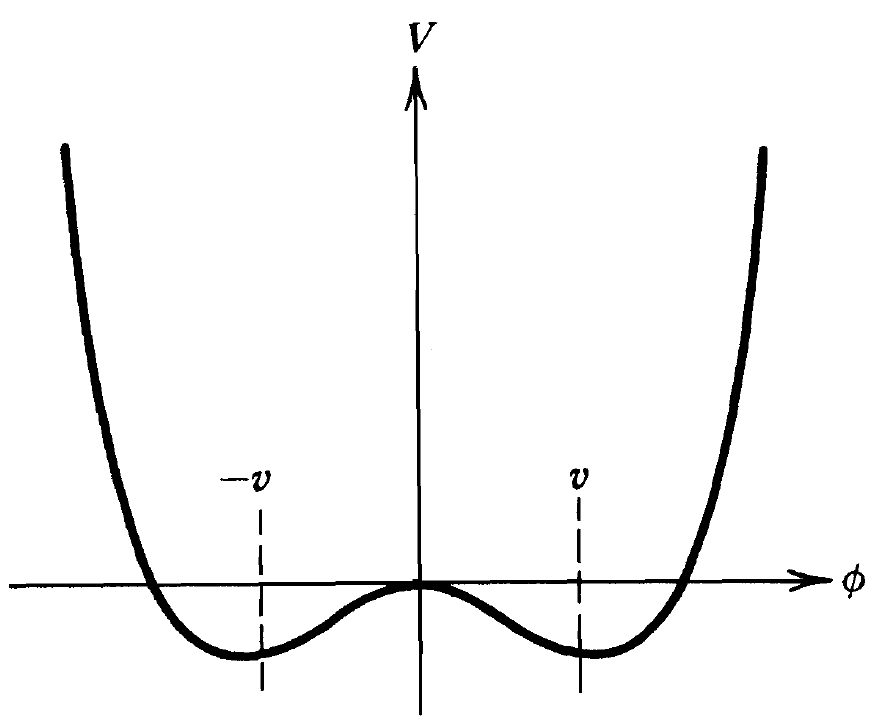
\includegraphics[width=0.5\textwidth]{figures/theory/Higgs_Field.png}
\caption{An example of one dimension ``Higgs'' potential \cite{Quark_Lepton}.}
  \label{fig:Higgs_Potential}
 \end{center}
\end{figure}

In perturbative calculation we should involve expansions around the minimum energy and this can be done by expanding the $\phi$ around the $v$
$$\phi(t,\mathbf{x})=v+h(t,\mathbf{x}).$$
It means $\phi$ can be expressed by $h$, while potential $V$ will not be symmetry under the change of $h$ to $-h$. This makes the ``spontaneous symmetry breaking'' of $\phi$. After expanding the $\phi$ around the VEV, in new Lagrangian we have a term related to the mass of $h$ (actually is the mass of ``Higgs'' boson) and a term related to the masses of gauge bosons which means the gauge bosons obtained the masses. By the way, the masses of fermions in SM are also ``generated'' by Higgs mechanism.

Last but not least, the only $SU(2)_L$ local symmetry does not create the physical $\mathrm{Z}$ boson. It is created together with $\mathrm{W^{\pm}}$ and photon in $SU(2)_L \times U(1)_Y$ (``Y'' means hypercharge, $Y=2Q-T^{3}$ with $Q$ is the charge of particle, $T^3$ is third component of weak-isospin) symmetry which is proposed by Weinberg, Salam, and Glashow \cite{PhysRevLett.19.1264,Salam1959,GLASHOW1959107}. This $SU(2)_L \times U(1)_Y$ gauge invariance theory unifies electromagnetic and weak interactions and is called electroweak theory. Finally, the complete SM theory is based on $SU(3)_c \times SU(2)_L \times U(1)_Y$ gauge symmetry.






\clearpage
\section{The Drell-Yan process}\label{sec:DY}
Due to its importance in this thesis for the search for heavy resonances in the dielectron final state (see Chapter \ref{chap:Zprime}), the Drell-Yan (DY) \cite{DRELL1971578} process is introduced with more details. The DY process is defined as the annihilation of a quark-antiquark pair into a pair of oppositely-charged leptons. The Feynman diagrams of the DY process at leading order are shown in Figure \ref{fig:DY12}. %These two amplitudes are proportional to the fine structure constant ($\alpha \approx 1/137$).

\begin{figure}[h!]
 \begin{center}
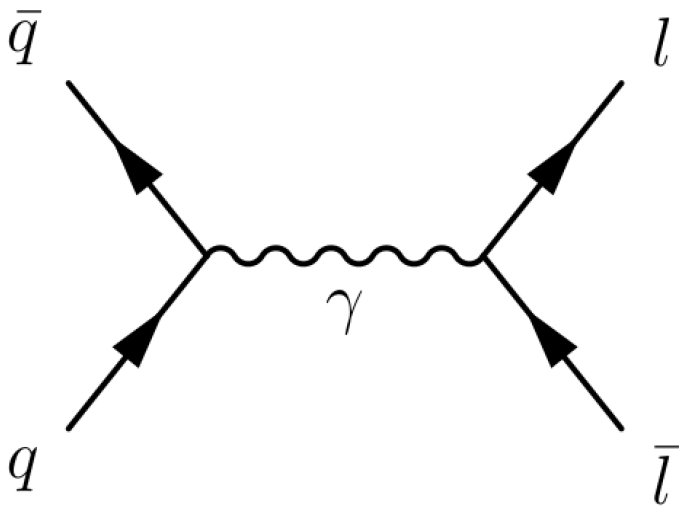
\includegraphics[width=0.4\textwidth]{figures/theory/DY1.png}
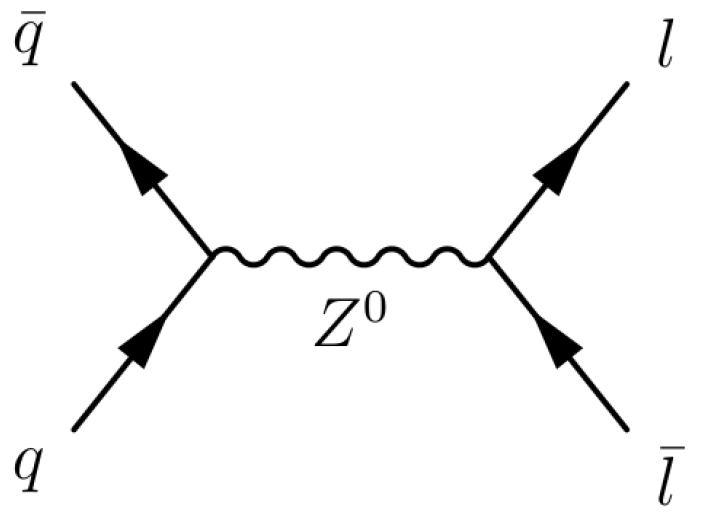
\includegraphics[width=0.4\textwidth]{figures/theory/DY2.png}
\caption{Feynman diagrams contributing to the Drell-Yan process at leading order. The left (right)
diagram corresponds to the annihilation of a $\mathrm{q\bar{q}}$ pair into a photon (a Z boson).}
  \label{fig:DY12}
 \end{center}
\end{figure}

The diagram in Figure \ref{fig:DY3}, with a Higgs boson exchange is neglected. Indeed, the coupling between the fermion and the Higgs boson is proportional to $m_{\mathrm{f}}/\upsilon$, where $m_{\textrm{f}}$ is the mass of the fermion and $\upsilon$ is the vacuum expected value of the scalar field ($\approx$ 246 GeV). So the amplitude of this diagram is proportional to $\frac{m_{\textrm{q}}\mathrm{(GeV)}}{246}\cdot\frac{m_{\mathrm{\ell}}\mathrm{(GeV)}}{246}$ with $m_{\mathrm{\ell}}$ be the mass of lepton. As we know, the valence quarks in the proton are the up and down quarks which are light ($m <$ 10 MeV).
%and it is hard to produce heavy sea quarks from gluons in the proton. 
Therefore the contribution of the third diagram is several orders of magnitude smaller than the first two diagrams in proton proton collision and it is usually neglected in the calculation.
\begin{figure}[h!]
 \begin{center}
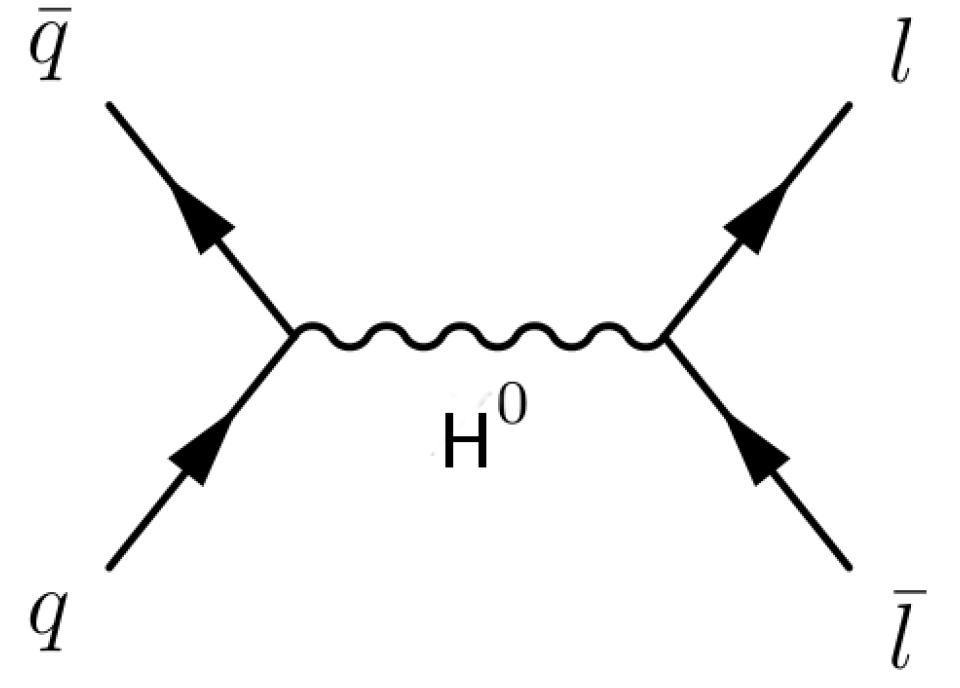
\includegraphics[width=0.4\textwidth]{figures/theory/DY3.png}
\caption{Feynman diagram of the process $\mathrm{q + \bar{q} \rightarrow H^{0} \rightarrow \ell + \bar{\ell}}$ at leading order.}
  \label{fig:DY3}
 \end{center}
\end{figure}

\subsection*{Cross-section}\label{subsec:DYxs}

The diagrams in Figure \ref{fig:DY12} give rise to two matrice terms $\mathcal{M}_{\gamma}$ and $\mathcal{M}_{\mathrm{Z}}$, hence the cross section of DY process can be expressed as:

\begin{equation}
\sigma_{\gamma/\mathrm{Z}}=\sigma_{\gamma} + \sigma_{\mathrm{Z}} + \sigma_{int}
\label{eq:sigma_DY}
\end{equation}

where $\sigma_{\gamma}$ is the cross-section corresponding to the exchange of a photon only,  $\sigma_{\mathrm{Z}}$ is for the exchange of a Z boson only, and $\sigma_{int}$ is the cross-section from the interference of the first two processes.

The formulas in the rest of the section are taken from \cite{Ellis_Webber}.

To be specific, the Equation \ref{eq:sigma_DY} can be written as:
\begin{equation}
\mathrm{\sigma(q(p_{1})\bar{q}(p_{2})\rightarrow l^{+}l^{-})=\frac{4\pi\alpha^{2}}{3s}\frac{1}{N}(Q_{q}^{2}-2Q_{q}V_{l}V_{q}\chi_{1}(s)+(A_{l}^{2}+V_{l}^{2})(A_{q}^{2}+V_{q}^{2})\chi_{2}(s))}
\label{eq:sigma_DY_detail}
\end{equation}
with
$$\mathrm{\chi_{1}(s)=\kappa\frac{s(s-M_{Z}^{2})}{(s-M_{Z}^{2})^{2}+\Gamma_{Z}^{2}M_{Z}^{2}}}$$
$$\mathrm{\chi_{2}(s)=\kappa^{2}\frac{s^{2}}{(s-M_{Z}^{2})^{2}+\Gamma_{Z}^{2}M_{Z}^{2}}}$$
$$\mathrm{\kappa=\frac{\sqrt{2}G_{F}M_{Z}^{2}}{16\pi\alpha}}$$

Here $\mathrm{p_{1}}$ is the four-momenta of the quark, $\mathrm{p_{2}}$ is the four-momenta of the anti-quark, and $\mathrm{s=(p_{1}+p_{2})^{2}}$. The $\alpha$ is the electromagnetic coupling, the $\mathrm{G_{F}}$ is the Fermi constant with the value $1.1663787\times10^{-5}~\mathrm{GeV}^{-2}$ \cite{FermiCon}, which can be precisely determined by muon lifetime experiment. The $\mathrm{M}_{\mathrm{Z}}$ and $\Gamma_{\mathrm{Z}}$ are the mass and total decay width of the Z boson respectively. The $\frac{1}{\mathrm{N}}=\frac{1}{3}$ and it is due to the color matching between quark and anti-quark. The $\mathrm{Q_{q}}$ is the charge of the quark, the $\mathrm{V}$ and $\mathrm{A}$ are the vectorial and axial couplings associated to the lepton/quark. The value of $\mathrm{V}$ and $\mathrm{A}$ are
$$\mathrm{V_{f}=T_{f}^{3}-2Q_{f}sin^{2}\theta_{W},~~~~A_{f}=T_{f}^{3}}$$
with $\mathrm{T_{f}}^{3}=+\frac{1}{2}$ for $\mathrm{f=\nu, u, ...}$ and $\mathrm{T_{f}}^{3}=-\frac{1}{2}$ for $\mathrm{f=e, d, ...}$. The $\mathrm{\theta_{W}}$ in $\mathrm{sin^{2}\theta_{W}}$ is so called ``weak mixing angle'' and it has been mathematically defined as $\mathrm{cos\theta_{W}=\frac{M_W}{M_Z}}$, here the $\mathrm{M_W}$ is the mass of W boson.

The first term ($\mathrm{\frac{4\pi\alpha^{2}}{3s}\frac{1}{N}Q_{q}^{2}}$) in the right side of Equation \ref{eq:sigma_DY_detail} is corresponding to $\sigma_{\gamma}$ and it can be calculated using QED. The second term ($\mathrm{\frac{4\pi\alpha^{2}}{3s}\frac{1}{N}(-2Q_{q}V_{l}V_{q}\chi_{1})}$) is for $\sigma_{int}$ and the last term ($\mathrm{\frac{4\pi\alpha^{2}}{3s}\frac{1}{N}(A_{l}^{2}+V_{l}^{2})(A_{q}^{2}+V_{q}^{2})\chi_{2}}$) is for $\sigma_{\mathrm{Z}}$.

From Equation \ref{eq:sigma_DY_detail} one can see that at low centra-mass of energy ($\sqrt{s}$) the Drell-Yan cross section is dominated by photon exchange process (e.g. at $\sqrt{s}=\mathrm{M_Z}/2$, the $\sigma_{\gamma}$ is around 100 times greater than $\sigma_{\mathrm{Z}}$ and over 10 times larger than $\sigma_{int}$), while at Z pole ($\sqrt{s}\sim \mathrm{M_Z}$) it is dominated by Z boson exchange process (e.g. at $\sqrt{s}=\mathrm{M_Z}$, the $\sigma_{\mathrm{Z}}$ is well over 100 times larger than $\sigma_{\gamma}$, while $\sigma_{int}$ is zero). To get a feeling about the Drell-Yan cross section as the function of lepton pair mass $\mathrm{M_{ll}}$ one can see Figure \ref{fig:DY_xs}.

\begin{figure}[h!]
 \begin{center}
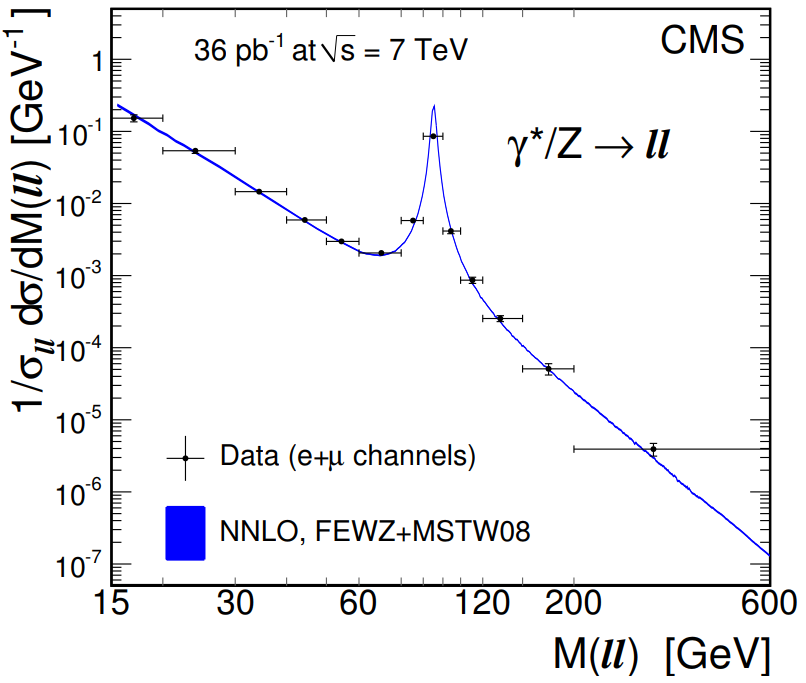
\includegraphics[width=0.9\textwidth]{figures/theory/DY_XS_CMS_Run1.png}
\caption{The normalized (in Z resonance region) DY cross section as the function of lepton pair mass ($\mathrm{M_{ll}}$) in $\mathrm{pp}$ collision at $\sqrt{s}=$ 7 TeV with CMS data \cite{Chatrchyan2011}.}
  \label{fig:DY_xs}
 \end{center}
\end{figure}

%\begin{figure}[h!]
% \begin{center}
%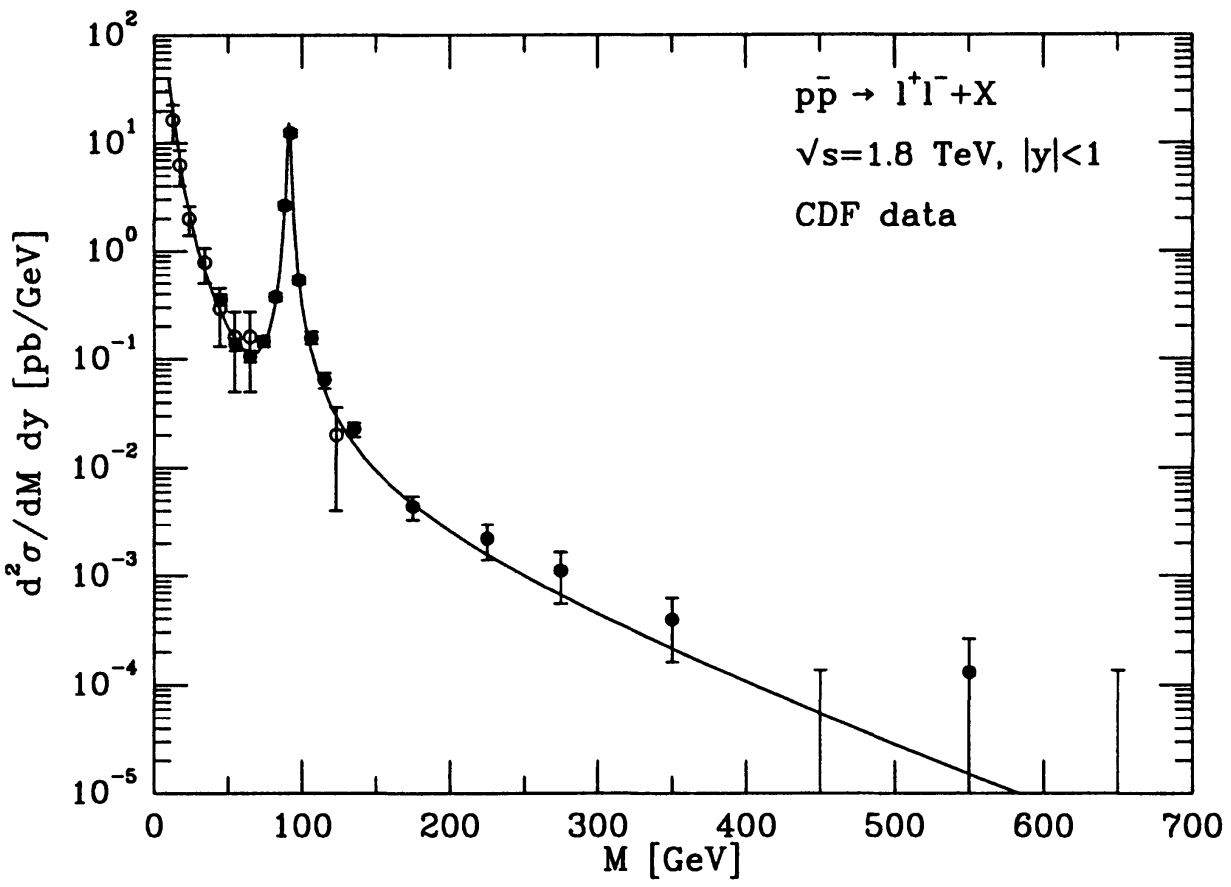
\includegraphics[width=0.9\textwidth]{figures/theory/DY_xs.png}
%\caption{The lepton pair cross section in $\mathrm{p\bar{p}}$ collision at $\sqrt{s}=$ 1.8 TeV with CDF data \cite{Ellis_Webber}.}
%  \label{fig:DY_xs}
% \end{center}
%\end{figure}


%\subsection{Partonic Cross-Section}\label{subsec:DYxs}
%
%The diagrams in Figure \ref{fig:DY12} give rise to two matrices terms $\mathcal{M}_{\gamma}$ and $\mathcal{M}_{Z}$, hence the cross section of DY process can be expressed as:
%
%\begin{equation}
%\sigma_{\gamma/Z}=\sigma_{\gamma} + \sigma_{Z} + \sigma_{int}
%\label{eq:sigma_DY}
%\end{equation}
%
%where $\sigma_{\gamma}$ is the cross-section corresponding to the creation of a photon only,  $\sigma_{Z}$ is for creating of a Z boson only and $\sigma_{int}$ is the cross-section from the interference of first two processes.
%
%The cross-section corresponding to the creation of a photon only can be written as \cite{Laurent_Thomas}:
%\begin{equation}
%\frac{d\sigma_{\gamma}}{d\Omega} = \frac{e^4}{(4 \pi)^2}Q^{2}_q Q^{2}_l\frac{1}{8s'} \left[ (1+ \cos\theta)^2 + (1 - \cos\theta)^2 \right]
%\label{eq:cs_photon}
%\end{equation}
%where $s'$ is the center-of-mass energy of the partonic process, $Q_{q,l}$ are the quark and lepton electrical charges and $\theta$ is defined as the angle between the quark and the negative lepton directions of flight in the $q\bar{q}$ center-of-mass frame. It can be observed that this cross-section remains the same for $\theta \rightarrow \pi - \theta  $.
%
%The cross-section corresponding to the creation of a Z boson only can be written as \cite{Laurent_Thomas}:
%\begin{equation}
%\frac{d\sigma_{Z}}{d\Omega} = \frac{e^4}{(4 \pi)^2} Q^{2}_q Q^{2}_l\frac{1}{8s'} |\mathcal{R}|^2  \left[ c_{1,Z}(1+ \cos\theta)^2 + c_{2,Z}(1 - \cos\theta)^2 \right]
%\label{eq:cs_z}
%\end{equation}
%where
%
%$$c_{1,Z}= ( (g_{V_l}^2+ g_{A_l}^2)(g_{V_q}^2+ g_{A_q}^2)+ 4g_{V_l} g_{A_l}g_{V_q}g_{A_q} )$$
%$$c_{2,Z}=((g_{V_l}^2+ g_{A_l}^2)(g_{V_q}^2+ g_{A_q}^2)- 4g_{V_l} g_{A_l}g_{V_q}g_{A_q} )$$
%$$\mathcal{R} = \left(\frac{1}{Q_l Q_q \sin^2 2\theta_W} \frac{1}{1 - M^2_Z/s' +i \Gamma_Z /M_Z}\right)$$
%
%and $g_V$ and $g_A$ are the vectorial and axial couplings associated to the lepton/quark.
%Because $c_{1,Z}$ and $c_{2,Z}$ are different, the cross-section is not invariant under $\theta \rightarrow \pi - \theta  $.
%The Z boson alone can therefore introduce a forward-backward asymmetry.
%% under the condition $g_{V_l}g_{A_l}g_{V_q}g_{A_q} \neq 0$, that is, no coupling vanishes.
%%It is also interesting to note that this term does not depend of the center-of-mass energy.
%
%The cross-section from the interference can be written as \cite{Laurent_Thomas}:
%\begin{equation}
% \frac{d\sigma_{int}}{d\Omega} = \frac{e^4}{(4 \pi)^2} Q^{2}_q Q^{2}_l\frac{1}{8s'} \text{Re}(\mathcal{R})  \left[ c_{1,int}(1+ \cos\theta)^2 + c_{2,int}(1 - \cos\theta)^2 \right]
%\label{eq:cs_int}
% \end{equation}
%where
%
%$$c_{1,int} =  2( g_{V_l} g_{V_q} + g_{A_l}g_{A_q} )$$
%$$c_{2,int}=  2  (g_{V_l} g_{V_q} - g_{A_l}g_{A_q} )$$
%again not invariant under $\theta \rightarrow \pi - \theta  $.
%
%The total angular differential cross-section, which is the sum of equations~(\ref{eq:cs_photon}),~(\ref{eq:cs_z}),~(\ref{eq:cs_int}), can be finally written as \cite{Laurent_Thomas}:
%\begin{equation}
% \frac{d\sigma_{\gamma / Z}}{d\Omega} = \frac{e^4}{(4 \pi)^2} Q^{2}_q Q^{2}_l\frac{1}{4s'}\left[ c_{1}(1+ \cos^2\theta) + c_{2} \cos\theta \right]
% \end{equation}
%where
%
%$$c_{1}= 1+ 2\text{Re}(\mathcal{R}) g_{V_l} g_{V_q}  + |\mathcal{R}|^2 (g_{V_l}^2+ g_{A_l}^2)(g_{V_q}^2+ g_{A_q}^2)$$
%$$c_{2}= 4\text{Re}(\mathcal{R}) g_{A_l} g_{A_q} + 8 |\mathcal{R}|^2 g_{V_l} g_{A_l}g_{V_q}g_{A_q}$$
%The total cross-section is \cite{Laurent_Thomas}:
%\begin{equation}
% \sigma_{\gamma / Z} =\int_\Omega  \frac{d\sigma_{\gamma / Z }}{d\Omega}  d\Omega =\frac{4\pi}{3}\frac{\alpha^2}{s'}c_1
%\label{eq:cs_tot}
% \end{equation}
%where $\alpha = e^2/(4\pi)$.
%\subsection{Forward-Backward Asymmetry}\label{sec:AFB}
%The definition of forward-backward asymmetry is given by \cite{Laurent_Thomas}:
%\begin{equation}
% A_{FB} = \frac{\sigma_{F}-\sigma_{B}}{\sigma_{F}+\sigma_{B}}= \frac{3}{8}\frac{c_2}{c_1}
%\end{equation}
%where $\sigma_{F} = \sigma_{\theta < \pi /2} $ is for forward cross-section and $\sigma_{B}=\sigma_{\theta > \pi /2}$ is for backward cross-section.
%
%So $A_{FB}=0$ means the cross-section is isotropic and $A_{FB}=1$ (or -1) corresponds to a purely forward (or backward) cross-section (the lepton is always closer to the quark/to the antiquark).
%
%This asymmetry strongly depends on $\sqrt{s'}$:
%\begin{itemize}
%\item[$\bullet$]At low $\sqrt{s'}$ (< 10 GeV) the photon contribution is dominant and the forward-backward asymmetry is then zero since the photon couples equally to left-handed and right-handed particles
%\item[$\bullet$]In the intermediate region it goes negative (mostly driven by the effect of the globally negative interference term)
%\item[$\bullet$]It's $\approx$ zero around the Z peak
%\item[$\bullet$]At high energy (above 100 GeV) it becomes a positive constant
%\end{itemize}
%
%This variable is of special interest in the search for new physics: the angular differential cross-section of any spin 1 particle is proportional to $(1+\cos^{2}(\theta)) + \frac{8}{3}A_{FB}\cos(\theta)$. The $A_{FB}$ can therefore help to distinguish signal from background or to identify a new signal \cite{Afb_paper}.

%\clearpage
\section{The photon induced process}\label{sec:PI}
As we known, the production of high invariant mass opposite sign lepton pairs in proton proton collision at the LHC is dominated by the Drell-Yan process (See previous section). Addition to this, photon-photon collisions, where the photons are radiated by the quarks in the proton, can also produce lepton pairs. The Feynman diagrams for the photon induced (PI) production of lepton pairs at leading order can be seen in Figure \ref{fig:PI}. The left diagram corresponds to a t-channel process and the right diagram corresponds to a u-channel process. There is no s-channel for the PI process at leading order and this will give different kinematic properties for the lepton pair comparing with Drell-Yan process which is s-channel.

\begin{figure}[h!]
 \begin{center}
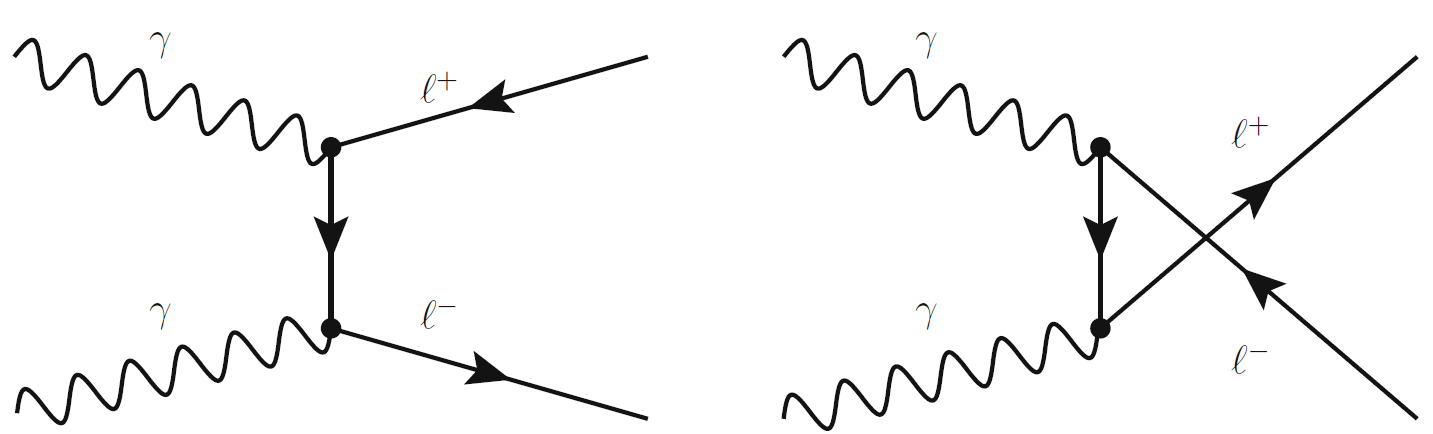
\includegraphics[width=0.9\textwidth]{figures/theory/PI.png}
\caption{Feynman diagrams for the photon induced production of lepton pairs at leading order. The left (right) diagram corresponds to a t-channel (u-channel) process.}
  \label{fig:PI}
 \end{center}
\end{figure}

The contribution from PI process becomes a significant part of the dilepton production at high invariant masses. Therefore, the knowledge of this process is important input for high mass resonant (like \ZP) or non-resonant searches. From \cite{PI_effect} we know the PI effects are generally small, not above the 5\% level, for masses of up to $\sim$ 2 TeV, but can reach $\sim$ 15�C20\% above 5 TeV. This effects will be taken into account in searching for \ZP study in Chapter \ref{chap:Zprime}.




\clearpage
\section{The effective field theory}\label{sec:EFT}
If new physics scale is reachable at the experiment then the new physics could be directly observed via the production of new particles.
Otherwise, it can take part in as a virtual particle which can not be detected directly but can still have an impact on the SM interactions by modifications of SM couplings or enhancements of rare SM processes.
In the latter case, the effective field theory (EFT) approach is useful to parameterize and constrain new physics.
In EFT, we extend the SM by adding new terms to the Lagrangian. An example of the extended Lagrangian is shown in Equation \ref{eq:EFT} where $\Lambda$ represents the energy scale beyond which new physics becomes relevant, $\mathcal{C}_{i}$ stands for the dimensionless Wilson coefficients (also called as the effective couplings), $\mathcal{O}_{i}^{6}$ are dimension-six operators.
Therefore, the underlying new physics particle gets integrated out (by measuring only $\mathcal{C}_{i}/\Lambda^{2}$) and leaving only the effective vertex, such as the Fermi theory for neutron decay (see the Feynman diagram in Figure \ref{fig:Neutron}). Besides, the EFT must maintain all the necessary symmetries of the SM. There are total O(100) new EFT vertices and it can be reduced by focusing on specific physical processes.

\begin{equation}
\mathcal{L}=\mathcal{L}_{SM} + \sum_{i}{\frac{\mathcal{C}_{i}}{\Lambda^{2}}\mathcal{O}_{i}^{6}}
\label{eq:EFT}
\end{equation}


\begin{figure}[h!]
 \begin{center}
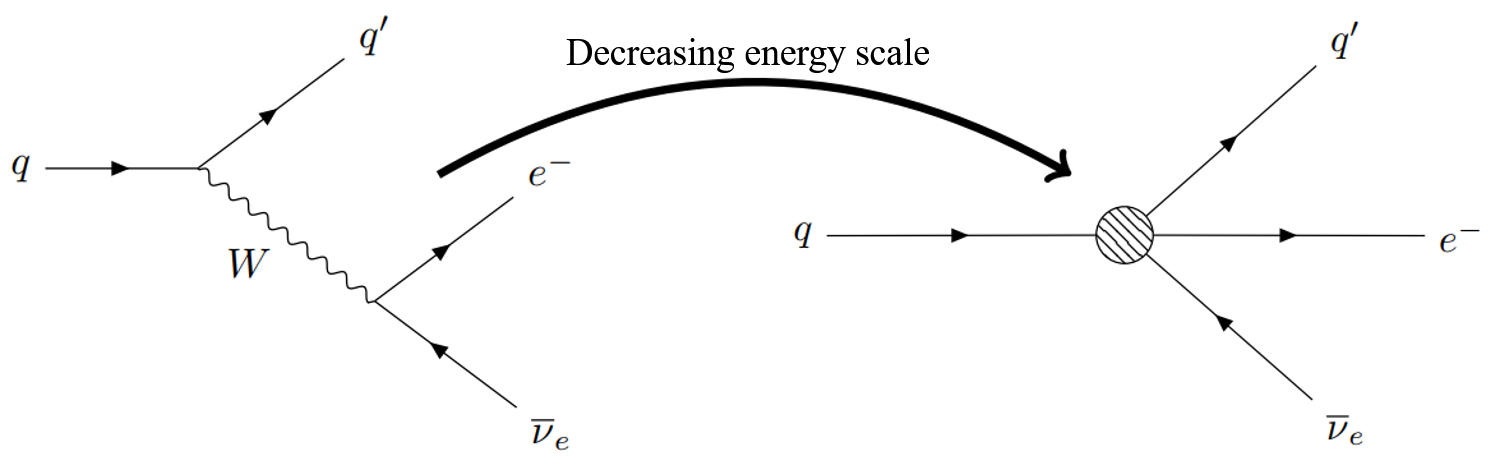
\includegraphics[width=0.75\textwidth]{figures/theory/Neutron.png}
\caption{The Feynman diagram for neutron decay for high energy scale (left) and low energy scale (right).}
  \label{fig:Neutron}
 \end{center}
\end{figure}


The EFT provides an important and powerful technique for searching for areas of new physics and it has the following properties:
\begin{enumerate}
\item It is a model independent approach, which means it does not depend on whatever the underlying new physics is. Therefore, it allows a systematically search for new physics in SM processes;
\item It is able to impose the same strict symmetry requirements as in the SM;
\item It can recover the full SM theory in a very natural way;
\item It can be used to quantify the accuracy with which new physics can be excluded.
\end{enumerate}

In this thesis the EFT approach is used for searching for new physics in top production which is reported in Chapter \ref{chap:tW}.

\section{Summary}
In this chapter, an introduction of the SM is delivered including the descriptions of the elementary particles and the three fundamental forces (electromagnetic, weak and strong). After that, a brief description about gauge symmetry is given. Due to its importance in this thesis, the Drell-Yan process is also introduced. Moreover, the photon induced dilepton production process is shortly discussed. Finally, a basic introduction about the effective field theory is given.

